\chapter{Selected Features}
\label{sec:user_features}

This chapter will give further insight on how to use some of the features of the
Visual Service Design Tool.  We subdivide those features into two groups: Features
for assisting in the modeling of Business Processes at a rather low level, and
features for managing a process model at a higher level, e.g. related to validating
and simulating processes.


%%%%%%%%%%%%%%%%%%%%%%%%%%%%%%%%%%%%%%%%%%%%%%%%%%%%%%%%%%%%%%%%%%%%%%%%%%%%%%%%
%%  Low-level Modeling Assistance                                             %%
%%%%%%%%%%%%%%%%%%%%%%%%%%%%%%%%%%%%%%%%%%%%%%%%%%%%%%%%%%%%%%%%%%%%%%%%%%%%%%%%

\section{Low-level Modeling Assistance}

The VSDT provides a number of features that help the user to quickly assemble a
business process diagram, such as both mouse-based and keyboard-based modeling
shortcuts.

%%%%%%%%%%%%%%%%%%%%%%%%%%%%%%%%%%%%%%%%%%%%%%%%%%%%%%%%%%%%%%%%%%%%%%%%%%%%%%%%

\subsection{GMF Modeling Assistance}

The \emph{Eclipse Graphical Modeling (GMF)} framework the VSDT is based upon
comes with a number of valuable modeling assistance features (if not desired,
modeling assistance can be turned off in the preferences).  In the following
some of these will be briefly introduced.  Figure~\ref{fig:modAss} is showing
the modeling assistance in use.

\begin{itemize}
	\item When resting the mouse on top of a compartment, a small palette will
	show up, showing the elements that can be placed in this compartment.  Thus
	one does not have to go all the way back to the palette for creating a new
	node.
	
	\item When resting the mouse on top of a node, small arrows going in and out
	of the node will appear.  By dragging these arrows new connections can be
	drawn.\footnote{Depending on the location, different connections will be
	offered: In the top and bottom region of a node incoming and outgoing Message
	Flows, in the left half incoming Sequence Flows and Associations, and in the
	right half outgoing Sequence Flows and Associations respectively.}
	
	\item When a connection is drawn and the mouse button is released over the
	canvas or another compartment, a node can be created in that place along with
	the connection.
	
	\item In case multiple node- or connection-types can be created using a given
	tool in a given context, the user will be prompted to select one.
\end{itemize}

\begin{figure}[ht]
	\centering
	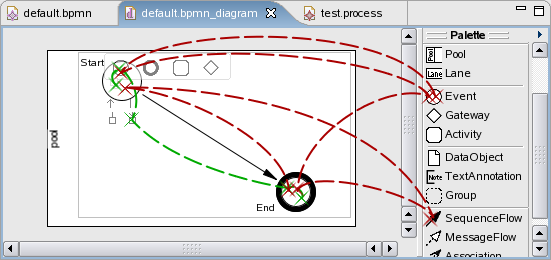
\includegraphics[width=.5\textwidth]{figures/features/modellingAssistant.png}
	\caption{Mouse movement with and without the use of the Modeling Assistant.}
	\label{fig:modAss}
\end{figure}

In case you do not like this feature, it can be disabled in the Preferences.


%%%%%%%%%%%%%%%%%%%%%%%%%%%%%%%%%%%%%%%%%%%%%%%%%%%%%%%%%%%%%%%%%%%%%%%%%%%%%%%%

\subsection{Appending Flow Objects}
Even faster than using the GMF modeling assistance, the \emph{Append} Actions can
be used for quickly appending new Flow Objects after existing ones.  It can be
reached through a Flow Object's context menu, or -- more conveniently -- by
using the keyboard shortcuts \texttt{Ctrl+Shift+(A|G|I|E)} for appending Activities,
Gateways, Intermediate and End Events.  Thus, after the first Start Event has
been placed, the basic workflow can quickly be assembled using only the Append
action and the TAB key to navigate between the existing nodes.


%%%%%%%%%%%%%%%%%%%%%%%%%%%%%%%%%%%%%%%%%%%%%%%%%%%%%%%%%%%%%%%%%%%%%%%%%%%%%%%%

\subsection{Connecting Flow Objects to a Sequence}
A group of Flow Objects can be selected and connected with Sequence Flows using
\emph{Connect to Sequence} Action or the keyboard shortcut \texttt{Ctrl+Shift+C}.
The Flow Objects will be connected in the order they have been selected.  Therefore
they should be selected one by one (holding down the Shift or Ctrl key), and not
using a selection margin.  This feature can be very useful when modeling a process
by first drawing a set of activities on the diagram and deciding later how to
arrange those activities to a working process.


%%%%%%%%%%%%%%%%%%%%%%%%%%%%%%%%%%%%%%%%%%%%%%%%%%%%%%%%%%%%%%%%%%%%%%%%%%%%%%%%

\subsection{Inserting Elements and Patterns}

By right-clicking on a Sequence Flow the \emph{Insert...} menu can be reached.
Here it is possible to insert a new element in between the source and the target
of that Sequence Flow, which is very useful for extending existing diagrams.  The
existing sequence Flow will be reoriented to the new element, preserving existing
attributes such as the condition, and a second Sequence Flow is drawn from the
new element to the existing Sequence Flow's former target.

Apart from basic elements such as Activities, Intermediate Events and Gateways,
it is also possible to insert complex workflow patterns, such as a split/merge
block or a loop.  This does not only greatly reduce the time needed for the
diagram creation\footnote{Reducing the pure editing time by up to 70\% according
to ~\cite{gschwind2008applying}.}, but also ensures that the workflow's structure
is sound (Referred to as ``correctness by construction'').

\emph{Note} that by now the layout of the diagram will not be adapted to the newly
inserted elements, thus the user will have to rearrange the surrounding elements
to make room for the new nodes.



%%%%%%%%%%%%%%%%%%%%%%%%%%%%%%%%%%%%%%%%%%%%%%%%%%%%%%%%%%%%%%%%%%%%%%%%%%%%%%%%
%%  Higher-level Process Management                                           %%
%%%%%%%%%%%%%%%%%%%%%%%%%%%%%%%%%%%%%%%%%%%%%%%%%%%%%%%%%%%%%%%%%%%%%%%%%%%%%%%%

\section{Handling non-visual Elements}

As noted earlier, the nodes, edges and labels visible in a Business Process
Diagram are just one half of the actual process model.  There are also a large
number of non-visual attributes to the visible elements and even entirely
non-visible elements, which are equally as important for the process.  The VSDT
provides a number of dialogs for managing those elements.


%%%%%%%%%%%%%%%%%%%%%%%%%%%%%%%%%%%%%%%%%%%%%%%%%%%%%%%%%%%%%%%%%%%%%%%%%%%%%%%%

\subsection{Dialogs for Handling Non-Visual Elements}

For each of the non-visual elements -- Properties, Assignments, Messages, and
Services -- there is a dedicated a management dialog.  The dialogs follow a
clear and recognizable layout, showing the elements as-is in a list along with a
number of buttons for inserting, removing and sorting of the elements and text
fields for editing the attributes of the currently selected item (see
Figure~\ref{fig:dialog}).

The various dialogs can be accessed in the following ways:
\begin{itemize}
	\item The \emph{Organize Properties Dialog} can be accessed via the context
	menu and property sheet of Pools, Activities and Message Flows, and by
	double-clicking an element in the BPMN-Properties View or a Message
	Flow.\footnote{In the case of Message Flows, the Properties of the underlying
	Message, if any, will be edited, and in the case of Pools, the Properties of
	the Pool's Process.}
	
	\item The \emph{Organize Assignments Dialog} can be accessed via the context
	menu and property sheet of Pools and Flow Objects, and by double-clicking
	Flow Objects.
	
	\item The \emph{Organize Message Channels Dialog} can be accessed via the
	property sheet of the Business Process Diagram.
	
	\item The \emph{Organize Services Dialog} can be accessed via the property
	sheet of the Business Process Diagram.
	
	\item The \emph{Organize Data Types Dialog} can be accessed via the property
	sheet of the Business Process Diagram.
\end{itemize}

\begin{figure}[ht]
	\centering
	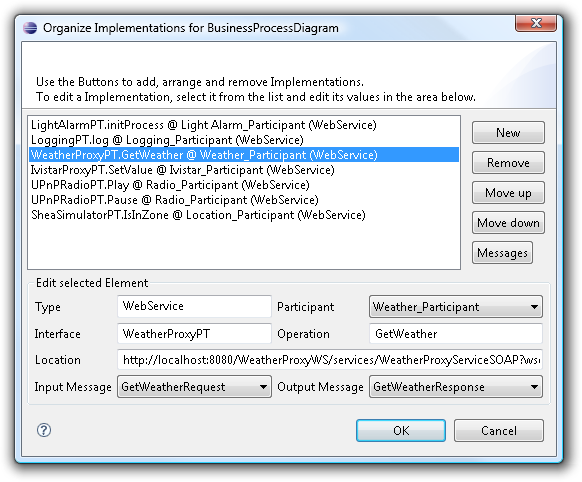
\includegraphics[width=.5\textwidth]{figures/features/dialog.png}
	\caption{A Supporting Type Organization Dialog.}
	\label{fig:dialog}
\end{figure}


%%%%%%%%%%%%%%%%%%%%%%%%%%%%%%%%%%%%%%%%%%%%%%%%%%%%%%%%%%%%%%%%%%%%%%%%%%%%%%%%

\subsection{Service Parameter Assignments}

While the \emph{Organize Assignments Dialog} provides means for organizing all
types of Assignments, it can be quite weary to make the assignments to a service
call, passing a number of values to the service's input parameters and storing
its results in other local variables.  Moreover, this is a common source for
mistakes, like selecting the wrong assign time, or missing an important input
parameter.  Using the \emph{Parameter Assignments Dialog} this task can be
facilitated in many ways.

\begin{figure}[ht]
	\centering
	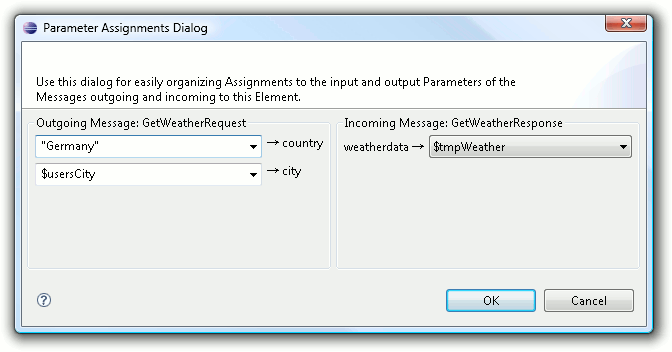
\includegraphics[width=.6\textwidth]{figures/features/paramAssign.png}
	\caption{Parameter Assignments Dialog}
	\label{fig:paramAssign}
\end{figure}

This dialog is available for all Activities and Events sending or receiving
messages, such as the Message Event and Send, Receive, Service and User Activity.
Provided that the Implementation and the input and output Messages for that
service are specified, the dialog displays a drop-down menu for each of the
incoming and/or outgoing Messages' Properties.  The values set in these lists
will then be used for the Assignments to the input and output parameters.  For
the outgoing message, arbitrary expressions can be inserted, while the parameters
of the incoming message can only be assigned to a local Property.  If more specific
Assignments are needed, the dialog can still be used for generating stubs for
those Assignments, which then can be refined in the \emph{Organize Assignments
Dialog}.  Further, the dialog will notify the user if there are input parameters
that have no value assigned to them.


%%%%%%%%%%%%%%%%%%%%%%%%%%%%%%%%%%%%%%%%%%%%%%%%%%%%%%%%%%%%%%%%%%%%%%%%%%%%%%%%

\subsection{Expressions}
\label{sec:user_features_exp}

The BPMN standard does not specify an expression language to be used.  Instead,
it is assumed that the language of the target framework is used, e.g.  XPath.
However, in a tool that provides transformations to various target frameworks
this is not an option.  While the diagram structure could be translated to the
syntax of the target system, the expression, given that they are written in an
unknown language, could not -- although all those languages might be very similar.
To address this flaw, the VSDT comes with its own, very simple expression language,
the \emph{VSDT Expression Language (VXL)}.  The advantage of using VXL is that it
provides a greatest common divisor of the expression languages used in the target
frameworks.  Thus, most expressions can be given using VXL, in which case they
can be validated and -- more importantly -- parsed and translated to the
respective expression languages used in the target frameworks.

\begin{figure}[ht]
	\centering
	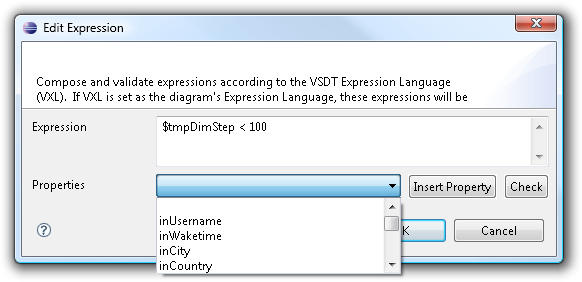
\includegraphics[width=.5\textwidth]{figures/features/editExp.png}
	\caption{The Edit Expression Dialog.}
	\label{fig:editExp}
\end{figure}

Each text field referring to an Expression in the dialogs and property sheets of
the VSDT provides a small button for opening the Edit Expression Dialog, which
can be seen in Figure~\ref{fig:editExp}.  This dialog not only provides a larger
text field for editing the Expression, but also a list of all the Properties visible
in the scope of the element owning the Expression, which can be selected from the
list and inserted into the expression.  Further, the \emph{Check} button can be
used to validate the Expression, which will check both the syntax and the
availability of the variables used in the expression.

\emph{Note} that there is no type checking yet.  However, this feature is on the
agenda, and will be implemented as soon as possible.



%%%%%%%%%%%%%%%%%%%%%%%%%%%%%%%%%%%%%%%%%%%%%%%%%%%%%%%%%%%%%%%%%%%%%%%%%%%%%%%%
%%  Higher-level Process Management                                           %%
%%%%%%%%%%%%%%%%%%%%%%%%%%%%%%%%%%%%%%%%%%%%%%%%%%%%%%%%%%%%%%%%%%%%%%%%%%%%%%%%

\section{Higher-level Process Management}

Finally, the VSDT provides a few features situated at a somewhat higher level,
such as validation and simulation, layout, process documentation or team-work.


%%%%%%%%%%%%%%%%%%%%%%%%%%%%%%%%%%%%%%%%%%%%%%%%%%%%%%%%%%%%%%%%%%%%%%%%%%%%%%%%

\subsection{Model Validation}

The VSDT provides two kinds of validation: Validation of BPMN constraints, and
structural validation.

\paragraph{Validation of Constraints}
BPMN diagrams can be checked to conform to the constraints given in the BPMN
specification by selecting \emph{Diagram $\rightarrow$ Validate} from the menu or
by clicking the checkmark icon in the tool bar.  Afterwards errors will be listed
in the problem view.  Additionally, faulty or otherwise problematic elements will
be marked with a respective icon in the process graph.

\paragraph{Structural Validation}
Besides the individual elements, also the structures in which these elements are
connected are important.  For checking the structure of the process, open the
Structure View (see Section \ref{sec:user_perspective_vsdtviews}) and click the
\emph{Structurize} button.  This will trigger the same Structure Mapping used in
the actual transformations (see Section~\ref{sec:user_trafo} and display the result,
i.e. a structured form of the process, featuring elements such as sequences and
blocks.  While the structured model might be a bit cumbersome to read, it gives
evidence of the structure that will be recognized from the process, and if this
is not the structure you intended you should consider restructuring the process.


%%%%%%%%%%%%%%%%%%%%%%%%%%%%%%%%%%%%%%%%%%%%%%%%%%%%%%%%%%%%%%%%%%%%%%%%%%%%%%%%

\subsection{Structure-Based Layout}

The Structure Mapping can also be used for calculating the layout of the BPMN
diagrams.  Compared to the layout algorithm provided by GMF, this proves especially
useful for diagrams containing upstream loops.  Still, since the structure-based
layout is still in an early stage, the default layout algorithm still is the one
provided by GMF.  The structure-based layout can be reached via the Structure
View (see Section~\ref{sec:user_perspective_vsdtviews}).

The recursive layout algorithm is sketched in algorithms~\ref{lst:layout1} and
\ref{lst:layout2}.  First, the process diagram is transformed to a block structure.
Then, the algorithm will step down into the structure and calculate the layout of
the ``blocks'' in a bottom-up way, taking the positions of the nested elements
into account.  The result of the algorithm is a map holding the bounding box for
each element, which can then be used for laying out the elements in the diagram
editor.

While the structure-based layout yields good results for well-structured diagrams,
i.e. diagrams that can be transformed to a block-structured form, the algorithms
is not applicable for non-structured diagram.

\begin{algorithm}
	\caption{\textsc{CreateLayoutMap}($diagram$)}
	\label{lst:layout1}
	\begin{algorithmic}
		\STATE $structuredDiagram \leftarrow \textsc{Structurize}(diagram)$
		\STATE $layoutMap \leftarrow $ create empty map
		\STATE $hint \leftarrow (0,~ 0)$
		\FOR{$pool$ in $structuredDiagram$}
			\STATE $box \leftarrow \textsc{CalculateBox}(pool,~ hint,~ layoutMap)$
			\STATE $hint \leftarrow (0,~ box.bottom)$
		\ENDFOR
		\RETURN $layoutMap$
	\end{algorithmic}
\end{algorithm}

\begin{algorithm}
	\caption{\textsc{CalculateBox}($element,~ topLeft,~ layoutMap$)}
	\label{lst:layout2}
	\begin{algorithmic}
		\STATE $hint \leftarrow topLeft$		
		\IF{$element$ is atomic}
			\STATE $box \leftarrow (topLeft.x,~topLeft.y,~\textsc{Width}(element),~\textsc{Height}(element))$
		\ELSE
			\IF{$element$ is sequence}
				\STATE $height \leftarrow 0$
				\FOR{$child$ in $element$}
					\STATE $box \leftarrow \textsc{CalculateBox}(child,~ hint,~ layoutMap)$
					\STATE $hint \leftarrow (box.left,~ box.top)$
					\STATE $height \leftarrow \textsc{Max}(height,~ box.height$
				\ENDFOR
				\STATE $box \leftarrow (topLeft.x,~ topLeft.y,~ hint.x - topLeft.x,~ height)$
			\ENDIF
			\STATE // similar for block, loop, subprocess, event handler, etc.
		\ENDIF
		\STATE insert $(element,~ box)$ into $layoutMap$
		\RETURN $box$
	\end{algorithmic}
\end{algorithm}


%%%%%%%%%%%%%%%%%%%%%%%%%%%%%%%%%%%%%%%%%%%%%%%%%%%%%%%%%%%%%%%%%%%%%%%%%%%%%%%%

\subsection{Visual Simulation and Interpretation}
\label{sec:user_features_sim}

BPMN diagrams created with the VSDT can be simulated and interpreted using the
built-in process interpreter (see Section~\ref{sec:user_perspective_vsdtviews}).
For starting a simulation, first switch to the BPMN diagram you want to simulate.
Open the \emph{Process Interpreter} view and click the \emph{Start} button.  For
each Pool in the diagram, the view will show those Activities that are currently
\textsc{active} or \textsc{ready}.  For advancing a step in the simulation, expand
a Pool and double-click one of the listed elements, that is the Flow Objects
currently being ready, e.g.\ its Start Events.  For more control, you can also
select one of \emph{Step Over}, \emph{Step Into} or \emph{Step Out}.  Hit the
Stop button for ending the simulation and removing the markers from the diagram
editor view.  In the diagram itself, the Flow Objects are annotated with a marker
symbol representing their state (see Table~\ref{tab:markerColors}).

\begin{table}[ht]
	\centering
	\caption{Mapping of Marker Colors to Flow Object States}
	\begin{tabular}{l|l}
		\bf Marker & \bf State of Flow Object       \\
		\hline
		Yellow    & Ready for execution             \\
		Blue      & Currently active / executing    \\
		Green     & Executed successfully            \\
		Red       & Execution failed or interrupted \\
		None      & Not yet executed or ready; idle \\
	\end{tabular}
	\label{tab:markerColors}
\end{table}

Once the simulation is running, the user can \emph{Step Over}, \emph{Step Into}
and \emph{Step Out} of Flow Objects.  Stepping into a Flow Object is particularly
interesting for Activities with attached Event Handlers or Embedded Subprocesses,
for which it is the default behavior.  Different kinds of interpretations are
available (or planned for the future):
\begin{itemize}
	\item \emph{Manual Simulation}: Here, the user is asked which way to proceed
	when coming to a branching point.  This mode is intended for presentation of
	documentary processes, but also for detecting e.g.\ deadlocks or other kinds
	of structural conflicts.
	
	\item \emph{Interpretation}: In this mode, Expressions used for instance in
	Assignments and Conditions are evaluated\footnote{Note that only Expressions
	given in the VSDT Expression Language (VXL) can be automatically evaluated,
	and that by now only simple data types are supported.} and stored, so that
	the process will automatically decide how to proceed at a branching point.
	Still, the user has to provide initial parameters and return values for
	service calls.  This mode is especially useful for testing the various
	Conditions and Assignments.
	
	\item \emph{Execution}: This mode integrates with a Service Directory, meaning
	that in addition to the \emph{Interpretation} mode, services used in the
	diagram will actually be invoked and their return values will be bound to the
	respective process properties.  Thus the user just has to provide the initial
	parameters of the process itself.  Apart from testing the interworking of the
	several services in the process, this mode can also be used for actually
	executing and monitoring the process. \emph{(work in progress)}
\end{itemize}


%%%%%%%%%%%%%%%%%%%%%%%%%%%%%%%%%%%%%%%%%%%%%%%%%%%%%%%%%%%%%%%%%%%%%%%%%%%%%%%%

\subsection{Text Generation}
\label{sec:user_features_text}
 
The VSDT features a powerful transformation of the Business Process Diagram to
natural language text.  Currently only English text is supported, but other
languages may be included in the future, as well.  The output text can have
different formats, e.g. plain text, HTML or Latex, which to use can be selected
in the Export Wizard.  While this feature is yet at an early stage, it can already
be used for quickly generating documentation for those who can not read the
process diagrams or for media where they are difficult to present, e.g. in a talk.
Emphasis has been laid on preserving the process structure as much as possible in
the text, e.g. using indentation.  Further a number of randomly selected redundant
terms is used to increase the linguistic diversity of the resulting text.

The Text Generation has been implemented using the same transformation framework
also used for code generation (see Section~\ref{sec:user_trafo}).  It can be
accessed via the \emph{Export} menu.


%%%%%%%%%%%%%%%%%%%%%%%%%%%%%%%%%%%%%%%%%%%%%%%%%%%%%%%%%%%%%%%%%%%%%%%%%%%%%%%%

\subsection{Import and Merging of Process Diagrams}

VSDT diagrams can be imported into and merged with each other.  While basically
this feature can be used for merging any two or more diagrams, it is most useful
for merging diverging versions of the same process diagram, having a common
ancestor.

After selecting \emph{Import other VSDT diagrams} from the Import menu, select
one or more diagrams to import \emph{from} and one diagram to import \emph{into}.
You can also check whether to create a backup of the original target file
(recommended), and whether the layout should be imported, too, or only the model
data, and whether the algorithm should try to merge identical elements.  The
latter, of course, only makes sense if the source and target files are different
revisions of the same process diagram.

The merging algorithm works by recursively comparing the \emph{ID}s of the objects
to be merged, so these should not be changed in different revisions.  Also there
are still some issues with conflicting changes, so one should always be sure to
create a backup and possibly use a \texttt{diff} tool to check whether the changes
to the file's XML source look plausible.


